%!TEX root = ../MasterThesis.tex

\section{Computer-Supported Cooperative Work}
\label{sec:cscw}

This section gives a short introduction to the theoretical foundations of \gls{CSCW} systems. It starts with an overview of the research field itself, followed by a description of the types of \gls{CSCW} systems available. After that it explains the concept of shared information spaces in detail.

\subsection{Fundamental aspects}
\label{sec:cscw_definition}

\gls{CSCW} is a \emph{generic} term that combines the understanding of the way people work in groups with the enabling technologies of computer networking, associated hardware, software, services and techniques. It is part of the research field of \emph{Cooperation Systems}, which emerged during the early 1980s with the understanding that a multi-disciplinary approach for \gls{IT} system design is needed for the success of such systems. As such the research field looks into the usage of applications to support group work in an organizational setting, the effects of such a system on the individual user, as well as how the applications have to be adapted for the context of the group. Therefore the studies of Cooperation Systems are consisting of a social part as well as a technical part, and are looking into the interrelationship between them for certain aspects of work in general, and explicitly for communication and cooperation in a team \citep{Grudin1994}.

% section cscw_defintion (end)

\subsection{Types of \gls{CSCW} systems}
\label{sec:cscw_types}

In a distributed team environment the style of communication could be \emph{synchronous} or \emph{asynchronous} depending on the dimension of time. If the communication takes place at the same time the communication is synchronous, otherwise asynchronous. Another aspect that needs to be taken into account is the place, which leads to the quadrant shown in Figure~\ref{fig:images_cscw_time_place_matrix}. \@

\begin{figure}[H]
 \centering
 %\includesvg[width=0.8\columnwidth, svgpath = images/]{cscw_time_place_matrix}
 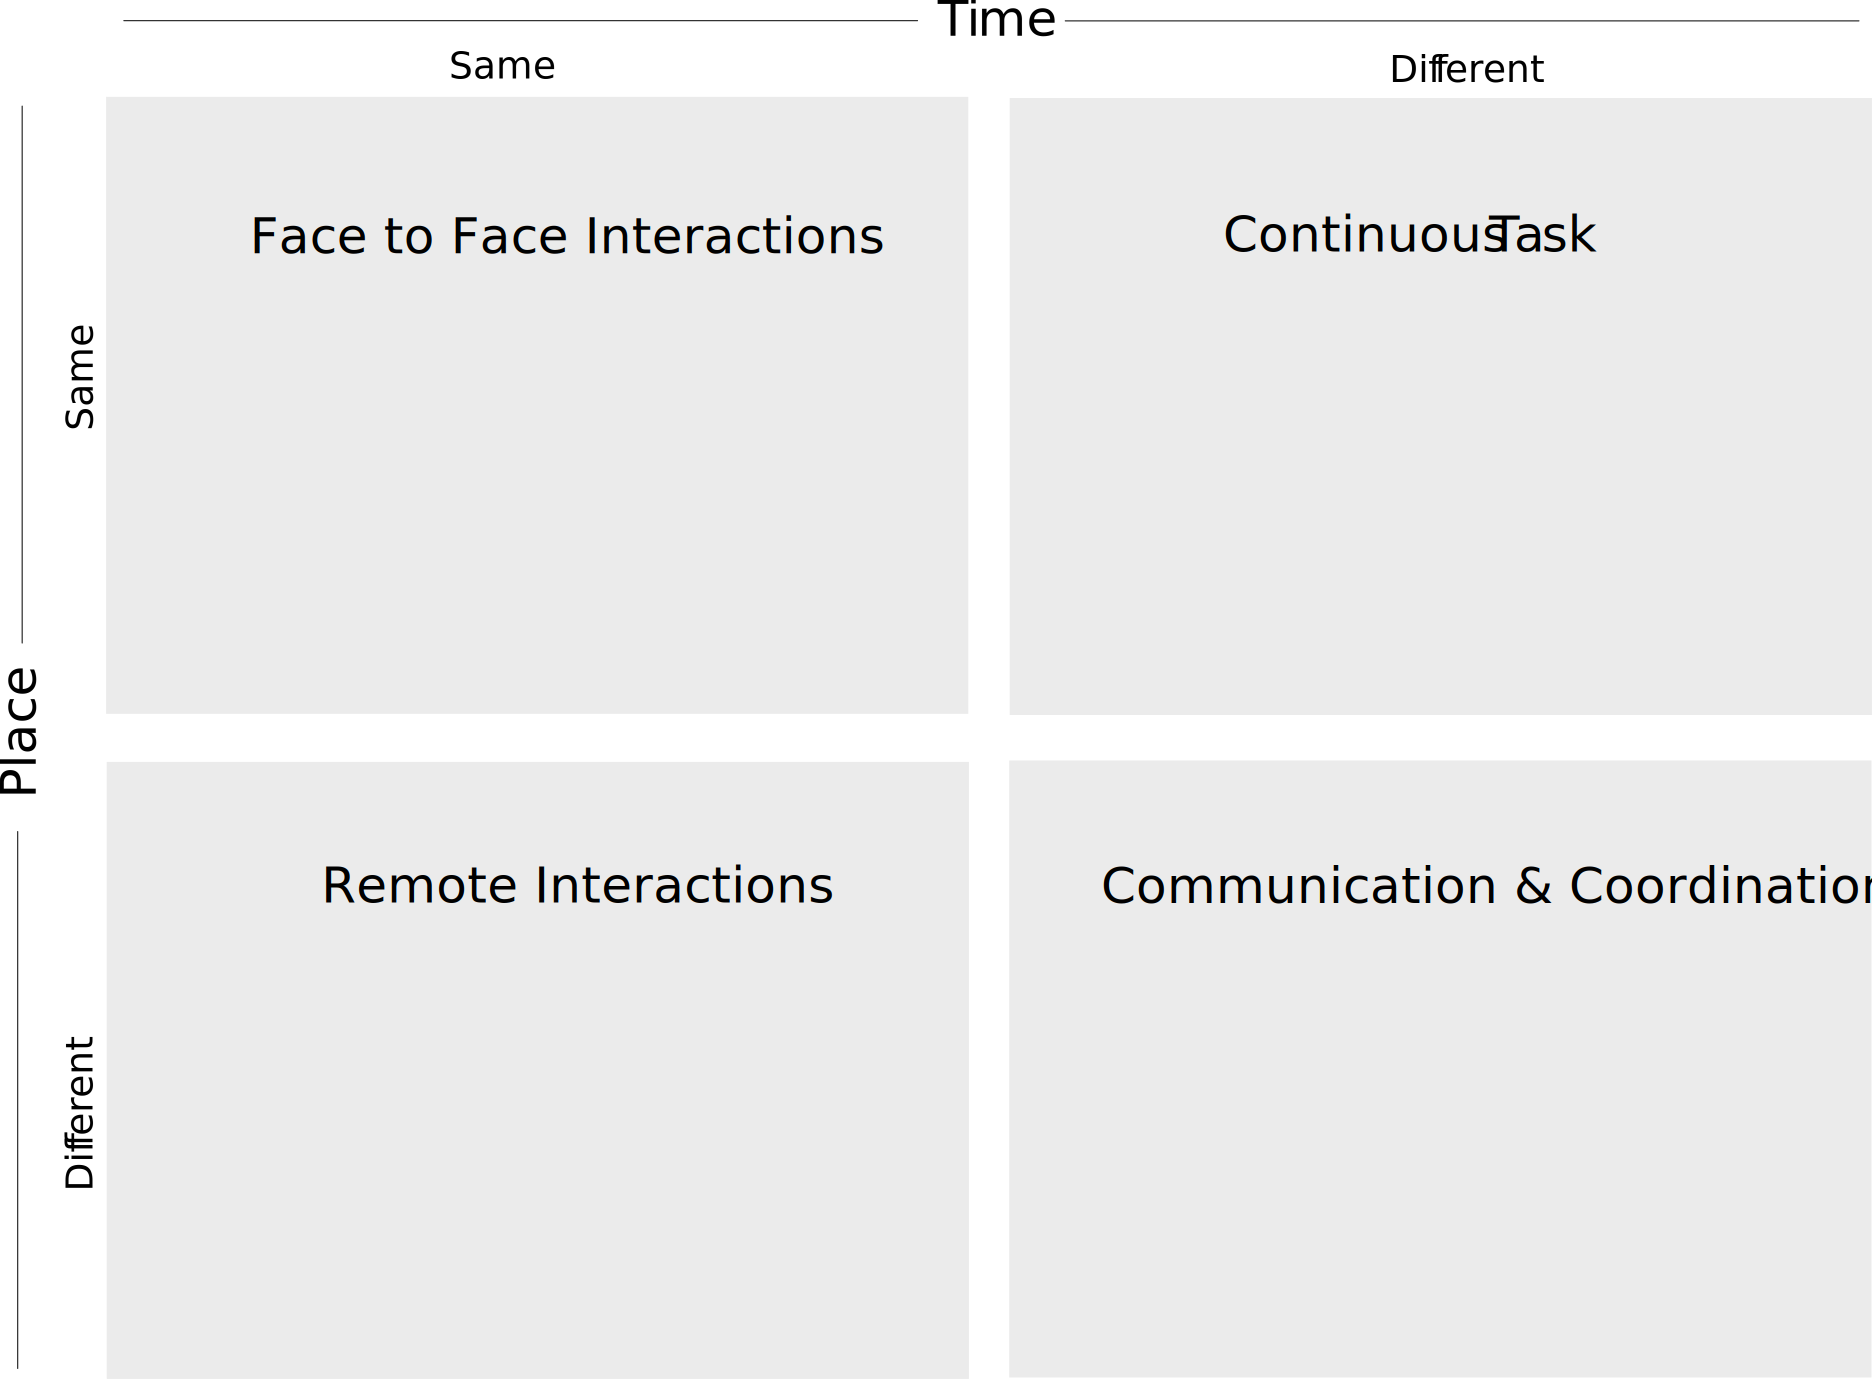
\includegraphics[width=0.8\columnwidth]{images/cscw_time_place_matrix.pdf}
 \caption[CSCW Place/Time Matrix]{\gls{CSCW} Place/Time Matrix \citep{xx}}
\label{fig:images_cscw_time_place_matrix}
\end{figure}

Additionally it is possible to group the CSCW systems based on the 3C model into \citep{Koch2008}:

\begin{itemize}
  \item \textbf{communication:} a two way exchange of information between different parties,
  \item \textbf{coordination:} management of shared resources such as meeting rooms, network printers, file shares, \ldots,
  \item \textbf{collaboration:} members of a group work together in a shared environment to reach a goal.
\end{itemize}

\begin{figure}[H]
 \centering
 %\includesvg[width=0.5\columnwidth, svgpath = images/]{cscw_time_place_matrix}
 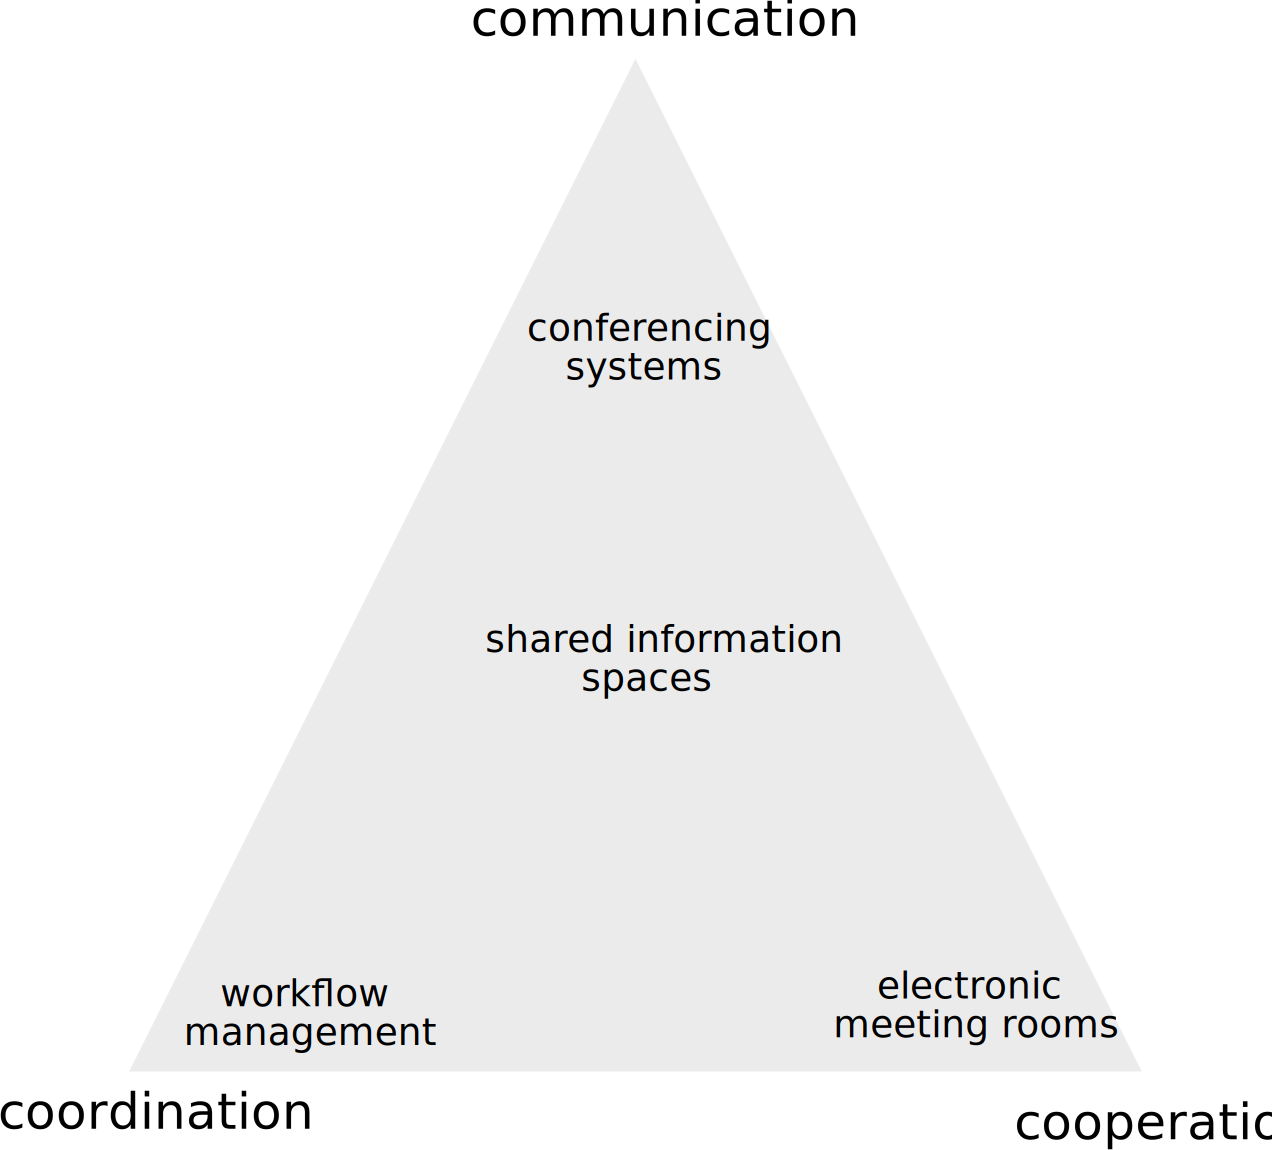
\includegraphics[width=0.8\columnwidth]{images/3C-model.pdf}
 \caption[The 3C Model]{The 3C Model \citep{Koch2008}}
\label{fig:images_cscw_3C_model}
\end{figure}

Typical examples might be (see also Figure~\ref{fig:images_cscw_3C_model}):

\begin{itemize}
  \item \textbf{group editors:} allows collaborated work on some kind of shared document or artefact; can face issues to keep the document in sync and setting up proper user roles and access rights,
  \item \textbf{shared information spaces:} also known as team rooms, cloud storage services, or document management systems that allow participants to access information at any place any time as well as to share information with others,
  \item \textbf{whiteboards:} allow multiple participants to work on a shared workspace and show the current and past activities of each of them; best used for ad-hoc brainstorming or idea generation.
\end{itemize}

% section cscw_types (end)

\subsection{Shared Information Spaces}
\label{sec:cscw_shared_spaces}

% section cscw_shared_spaces (end)

% section cscw (end)
